\hypertarget{ux8bbfux95eeux6570ux636eux5e93}{%
\subsection{访问数据库}\label{ux8bbfux95eeux6570ux636eux5e93}}

程序运行的时候,数据都是在内存中的。当程序终止的时候,通常都需要将数据保存到磁盘上,无论是保存到本地磁盘,还是通过网络保存到服务器上,最终都会将数据写入磁盘文件。

而如何定义数据的存储格式就是一个大问题。如果我们自己来定义存储格式,比如保存一个班级所有学生的成绩单:

\begin{longtable}[]{@{}ll@{}}
\toprule
名字 & 成绩 \\ \addlinespace
\midrule
\endhead
Michael & 99 \\ \addlinespace
Bob & 85 \\ \addlinespace
Bart & 59 \\ \addlinespace
Lisa & 87 \\ \addlinespace
\bottomrule
\end{longtable}

你可以用一个文本文件保存,一行保存一个学生,用\texttt{,}隔开:

\begin{pythoncode}
Michael,99
Bob,85
Bart,59
Lisa,87
\end{pythoncode}

你还可以用 JSON 格式保存,也是文本文件:

\begin{pythoncode}
[
    {"name":"Michael","score":99},
    {"name":"Bob","score":85},
    {"name":"Bart","score":59},
    {"name":"Lisa","score":87}
]
\end{pythoncode}

你还可以定义各种保存格式,但是问题来了:

存储和读取需要自己实现,JSON 还是标准,自己定义的格式就各式各样了;

不能做快速查询,只有把数据全部读到内存中才能自己遍历,但有时候数据的大小远远超过了内存(比如蓝光电影,40GB
的数据),根本无法全部读入内存。

为了便于程序保存和读取数据,而且,能直接通过条件快速查询到指定的数据,就出现了数据库(Database)这种专门用于集中存储和查询的软件。

数据库软件诞生的历史非常久远,早在 1950
年数据库就诞生了。经历了网状数据库,层次数据库,我们现在广泛使用的关系数据库是
20 世纪 70 年代基于关系模型的基础上诞生的。

关系模型有一套复杂的数学理论,但是从概念上是十分容易理解的。举个学校的例子:

假设某个 XX 省 YY 市 ZZ 县第一实验小学有 3 个年级,要表示出这 3
个年级,可以在 Excel 中用一个表格画出来:

 
 \begin{figure}[htp]
	\centering
	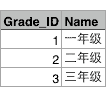
\includegraphics[width=0.6\linewidth]{fig/9466582752136320.png}
\end{figure}


每个年级又有若干个班级,要把所有班级表示出来,可以在 Excel
中再画一个表格:

 
 \begin{figure}[htp]
	\centering
	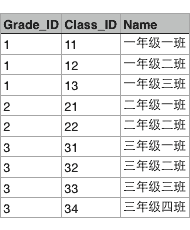
\includegraphics[width=0.6\linewidth]{fig/9466583066904000.png}
\end{figure}


这两个表格有个映射关系,就是根据 Grade\_ID
可以在班级表中查找到对应的所有班级:

 
 \begin{figure}[htp]
	\centering
	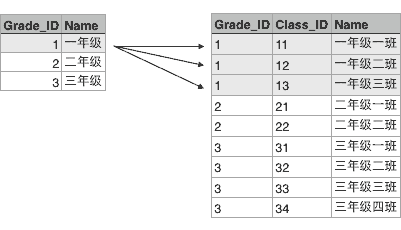
\includegraphics[width=0.6\linewidth]{fig/9466584239922880.png}
\end{figure}


也就是 Grade 表的每一行对应 Class
表的多行,在关系数据库中,这种基于表(Table)的一对多的关系就是关系数据库的基础。

根据某个年级的 ID 就可以查找所有班级的行,这种查询语句在关系数据库中称为
SQL 语句,可以写成:

\begin{pythoncode}
SELECT * FROM classes WHERE grade_id = '1';
\end{pythoncode}

结果也是一个表:

\begin{pythoncode}
---------+----------+----------
grade_id | class_id | name
---------+----------+----------
1        | 11       | 一年级一班
---------+----------+----------
1        | 12       | 一年级二班
---------+----------+----------
1        | 13       | 一年级三班
---------+----------+----------
\end{pythoncode}

类似的,Class 表的一行记录又可以关联到 Student 表的多行记录:

 
 \begin{figure}[htp]
	\centering
	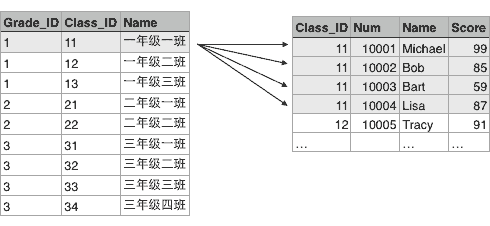
\includegraphics[width=0.6\linewidth]{fig/9466587096437760.png}
\end{figure}


由于本教程不涉及到关系数据库的详细内容,如果你想从零学习关系数据库和基本的
SQL 语句,如果你想从零学习关系数据库和基本的 SQL 语句,请参考
\href{https://www.liaoxuefeng.com/wiki/1177760294764384}{SQL 教程}。

\hypertarget{nosql}{%
\subsubsection{NoSQL}\label{nosql}}

你也许还听说过 NoSQL 数据库,很多 NoSQL
宣传其速度和规模远远超过关系数据库,所以很多同学觉得有了 NoSQL
是否就不需要 SQL 了呢?千万不要被他们忽悠了,连 SQL
都不明白怎么可能搞明白 NoSQL 呢?

\hypertarget{ux6570ux636eux5e93ux7c7bux522b}{%
\subsubsection{数据库类别}\label{ux6570ux636eux5e93ux7c7bux522b}}

既然我们要使用关系数据库,就必须选择一个关系数据库。目前广泛使用的关系数据库也就这么几种:

付费的商用数据库:

\begin{itemize}
\item
  Oracle,典型的高富帅;
\item
  SQL Server,微软自家产品,Windows 定制专款;
\item
  DB2,IBM 的产品,听起来挺高端;
\item
  Sybase,曾经跟微软是好基友,后来关系破裂,现在家境惨淡。
\end{itemize}

这些数据库都是不开源而且付费的,最大的好处是花了钱出了问题可以找厂家解决,不过在
Web
的世界里,常常需要部署成千上万的数据库服务器,当然不能把大把大把的银子扔给厂家,所以,无论是
Google、Facebook,还是国内的 BAT,无一例外都选择了免费的开源数据库:

\begin{itemize}
\item
  MySQL,大家都在用,一般错不了;
\item
  PostgreSQL,学术气息有点重,其实挺不错,但知名度没有 MySQL 高;
\item
  sqlite,嵌入式数据库,适合桌面和移动应用。
\end{itemize}

作为 Python 开发工程师,选择哪个免费数据库呢?当然是 MySQL。因为 MySQL
普及率最高,出了错,可以很容易找到解决方法。而且,围绕 MySQL
有一大堆监控和运维的工具,安装和使用很方便。

为了能继续后面的学习,你需要从 MySQL 官方网站下载并安装
\href{http://dev.mysql.com/downloads/mysql/}{MySQL Community Server
5.6},这个版本是免费的,其他高级版本是要收钱的(请放心,收钱的功能我们用不上)。

